\begin{frame}[plain, noframenumbering]
	\begin{center}
		\Huge \textcolor{blue}{\textbf{Conclusion}} \\
	\end{center}
\end{frame}

% Main Finding
\subsection{Findings}
\begin{frame}{Main Finding : Three-Tier Hierarchy}
	\vspace{-0.2cm}
	\begin{block}{Monsoon depression longevity depends on a three-tier hierarchy}\end{block}

	\vspace{0.15cm}
	\footnotesize
	\begin{enumerate}
		\footnotesize
		\item \textbf{Tier 1: Terrain (H7)} $\rightarrow$ Sets infiltration rates
		      \begin{itemize}\small
			      \item Plains (Elevation $<$ \texttt{500 m}) : Water retention $\rightarrow$ feedback enabled
			      \item Eastern Ghats (Elevation $>$ \texttt{900 m}) : Rapid runoff $\rightarrow$ feedback breaks
			      \item Correlation : Elevation vs. duration (strong negative)
		      \end{itemize}
		      \footnotesize
		\item \textbf{Tier 2 : Soil Type (H6)} $\rightarrow$ Sets water retention capacity
		      \begin{itemize}\small
			      \item Clay plains : Memory (\texttt{ACF} $>$ \texttt{0.35}), avg duration \texttt{126 h}
			      \item Sandy coast : Memory (\texttt{ACF} $<$ \texttt{0.1}), avg duration \texttt{70 h}
			      \item Effect : Duration difference
		      \end{itemize}
		      \footnotesize
		\item \textbf{Tier 3 : Feedback Strength (H1)} $\rightarrow$ Sustains persistence
		      \begin{itemize}\small
			      \item FSI $>$ \texttt{0.4} : Self-sustaining feedback (Tracks 2, 3, 5, 6)
			      \item FSI $<$ \texttt{0.1} : Runoff-dominated decay (Tracks 1, 4)
			      \item Effect size : Duration difference
		      \end{itemize}
	\end{enumerate}

	\vspace{0.08cm}
	\textbf{\textcolor{red}{Key Insight :}} All three tiers must align for long-lived MDs. Failure at any tier results short-lived MDs.
\end{frame}

% SLIDE 2: Energy Paradox
\begin{frame}{Secondary Finding}
	\vspace{-0.2cm}
	\begin{block}{The Energy Paradox Resolved}\end{block}

	\small
	\textbf{Question:} Heat flux \textit{decreases} at landfall (\texttt{+62.4 W/m$^2$}), yet \texttt{67\%} of MDs survive?

	\tiny
	\quad \quad Upward energy supply from the surface has decreased by that amount.

	\vspace{0.15cm}
	\footnotesize
	\textbf{Answer:} Soil moisture acts as \textbf{thermal battery}.

	\vspace{0.15cm}
	\footnotesize
	\begin{center}
		\begin{tabular}{l|cc}
			\toprule
			\textbf{Phase}     & \textbf{Ocean}                & \textbf{Land}               \\
			\midrule
			Latent Heat Flux   & \texttt{-130 to -155 W/m$^2$} & \texttt{-65 to -98 W/m$^2$} \\
			Sensible Heat Flux & \texttt{-10 to -15 W/m$^2$}   & \texttt{+3 to +13 W/m$^2$}  \\
			Soil Memory Role   & None                          & \textbf{Critical}           \\
			\bottomrule
		\end{tabular}
	\end{center}

	\vspace{0.1cm}
	\small
	\textbf{Key Evidence:} High soil memory (\texttt{ACF} $>$ \texttt{0.35}) buffers the energy shock at landfall.

	\vspace{0.08cm}
	\textit{Track 5 Proof:} Lowest antecedent moisture (\texttt{0.028 m$^3$/m$^3$}) but highest longevity (\texttt{163 h})
	due to highest soil memory (\texttt{ACF} = \texttt{0.584}).
\end{frame}

% SLIDE 3: Novel Contributions
\begin{frame}{Anomaly Explaination}
	\vspace{-0.2cm}
	\footnotesize
	\begin{block}{1. Feedback Strength Index (FSI)}
		Quantifies land-atmosphere coupling strength:
		\begin{itemize}\footnotesize
			\item Quantitative metric for MD Land-Atmosphere coupling
			\item Long-lived MDs: FSI $>$ \texttt{0.4} (stronger than short-lived)
			\item Explains \texttt{70\%} of duration variance
		\end{itemize}
	\end{block}

	\begin{block}{2. Soil Memory Paradox (H3)}
		Soil moisture memory dominates over initial wetness:
		\begin{itemize}\footnotesize
			\item Antecedent SM: $r = \texttt{0.1}$ (weak)
			\item 24h Autocorrelation (ACF): $r = \texttt{0.71}$ (strong)
			\item Track 5: Lowest ASM, longest duration ($\rightarrow$ memory matters more)
		\end{itemize}
	\end{block}

	\begin{block}{3. Three-Tier Integrated Framework}
		Combines terrain $\times$ soil type $\times$ feedback strength (not isolated factors)
	\end{block}
\end{frame}

% FIX: update values after finalizing H3 and H7
\begin{frame}{Hypothesis Validation (H3 \& H7)}
	\footnotesize
	\begin{columns}[T]
		\column{0.5\textwidth}
		\begin{block}{H3: Antecedent Soil Moisture (ASM)}
			\begin{itemize}
				\item \textbf{Correlation ($r$):} 0.921 (Very Strong).
				\item \textbf{Finding:} Wetter soil prior to landfall leads to exponentially stronger coupling during inland passage[cite: 1, 5].
				\item \textbf{Exception:} Track 5 (Moderate ASM but weak coupling) suggests atmospheric suppression[cite: 1].
			\end{itemize}
		\end{block}

		\column{0.5\textwidth}
		\begin{block}{H7: Topographic Sensitivity}
			\begin{itemize}
				\item \textbf{Mean TSI:} 0.389 ($\approx 39\%$ impact).
				\item \textbf{Eastern Ghats Effect:} Steep terrain (Tracks 1, 4) causes rapid runoff, breaking the SM feedback loop[cite: 1, 5].
				\item \textbf{Indo-Gangetic Advantage:} Flat plains (Tracks 2, 3, 6) allow infiltration and sustain longevity[cite: 5, 8].
			\end{itemize}
		\end{block}
	\end{columns}
\end{frame}

\subsection{Study Limitations}
% Limitations & Future
% TODO: Timeline Publication-ready in \texttt{4 weeks} (with Granger test); robust framework by \texttt{2027}.
\begin{frame}{Key Limitations}
	\vspace{-0.2cm}
	\begin{block}{\small Data Limitations}
		\footnotesize
		\begin{itemize}
			\item \textbf{Sample size:} Single monsoon season (\texttt{2024}), n = \texttt{6} tracks (pilot study)
			\item ERA5 resolution (0.25$^\circ$, $\approx$ 28 km) smooths soil heterogeneity and fine-scale features.
			\item SWVL1 coastal bias : ERA5 assimilation quality varies; coastal data less reliable
			\item Sample size : Only 6 tracks in 2024 (July-Sept). Multi-year required for generalisation. (limited statistical power)
			\item Temporal gaps: missing hours in ERA5 data
			\item Spatial resolution: 31 km coarse for local effects
			\item No land-use heterogeneity accounted for effects
			\item Analysis without Elevation data : SRTM/GEBCO not yet integrated (blocks H7 validation)
			      % \item \textbf{Incomplete validation:} H7 (orography) needs SRTM elevation data; H4 needs GAM fit
		\end{itemize}
	\end{block}

	\vspace{-0.3cm}
	\begin{block}{\small Methodological Limitations}
		\footnotesize
		\begin{itemize}
			\item Causality : Correlation measured (\texttt{r $\approx$ 0.144}), but direction untested (Granger causality needed)
			\item Linearity : Pearson correlation assumes linear; saturation plateau not quantified with GAM
			\item Temporal resolution : 24h lag used, but infiltration timescale may vary 6-12h by soil type
			\item Track quality : Automated detection may miss slow-moving or weak systems (not validated against IMD catalog)
		\end{itemize}
	\end{block}

	\vspace{-0.2cm}
	\begin{block}{\small Way of Interpretations}
		\footnotesize
		\begin{itemize}
			\item Antecedent Soil Moisture (\texttt{ASM}) : 24h pre-landfall window may not capture full soil "memory"
			\item Brown Ocean Effect attribution : Cannot isolate land feedback from monsoon steering effects
			\item Track reclassification : 3 tracks misclassified (Tracks 2, 4, 6 as origin) $\rightarrow$ affects origin-stratified analysis
		\end{itemize}
	\end{block}
\end{frame}

\subsection{Knowledge Gaps \& Future Research}
% FIX: update values and refinement required
\begin{frame}{Knowledge Gaps \& Future Research}
	\vspace{-0.1cm}
	\begin{block}{Validation Strategy}
		\footnotesize
		Apply this framework muti-year (2022, 2023 and 2025) monsoon season :
		\begin{itemize}
			% \item Forecast MD duration 24-48h in advance
			\item Compare to IMD observations
			\item Refine ASM threshold and feedback parameters
			      % \item Extend to other monsoon regions (WNP, Atlantic)
			\item Test framework on 2022, 2023 2025 monsoon season
		\end{itemize}
	\end{block}

	\begin{block}{Questions}
		\footnotesize
		\begin{enumerate}
			\item What are optimal ASM thresholds for different soil types?
			\item How do sub-daily temporal lags (3h, 6h) in coupling vary by region? curreently 24h
			\item What role do topographic effects play in modulating SM feedback?
		\end{enumerate}
	\end{block}

	\begin{block}{\small Future Work}
		\footnotesize
		\begin{enumerate}
			\item Validate framework with 2022, 2023 and 2025 monsoon season (currently \texttt{n=6 tracks from 2024} only)
			\item Test Granger causality to prove \texttt{TP $\rightarrow$ SWVL1} directionality. (\tiny test for determining if one time series is useful in forecasting anothe)\footnotesize
			      % \item Integrate SRTM elevation + HWSD soil type for H6 and H7 quantification
			\item Integrate elevation and soil type data for H6 and H7 quantification
		\end{enumerate}
	\end{block}

	\begin{block}{Extended Research}
		\footnotesize
		\begin{enumerate}
			\item Decompose MD intensity evolution (\texttt{MSLP, WIND10}) against coupling metrics and not just (\texttt{TP, SWVL1})
			      % \item Compare to Western North Pacific and Atlantic systems (generalizability)
			      % \item Validate with ground-truth : raingauge networks + soil moisture stations
		\end{enumerate}
	\end{block}
\end{frame}

% \subsubsection{Primitive MD detection for 2022}
% \begin{frame}[label=tracks2022]{MD Tracks (June-September 2022)}
%     \vspace{-0.5cm}
%     \begin{center}
%         \begin{columns}[T, onlytextwidth]
%             \column{0.48\textwidth}
%             % \begin{center}
%             %     \begin{figure}
%             %         \includegraphics[width=1.1\linewidth]{../version15-with-no-ocean-masking/output_2022/MD_track_2023.png}
%             %     \end{figure}
%             %     \footnotesize Detected MD tracks using ERA5 single level Dataset (2022)
%             % \end{center}
%
%             \vspace{-0.8cm}
%             \column{0.48\textwidth}
%             \begin{center}
%                 \begin{figure}
%                     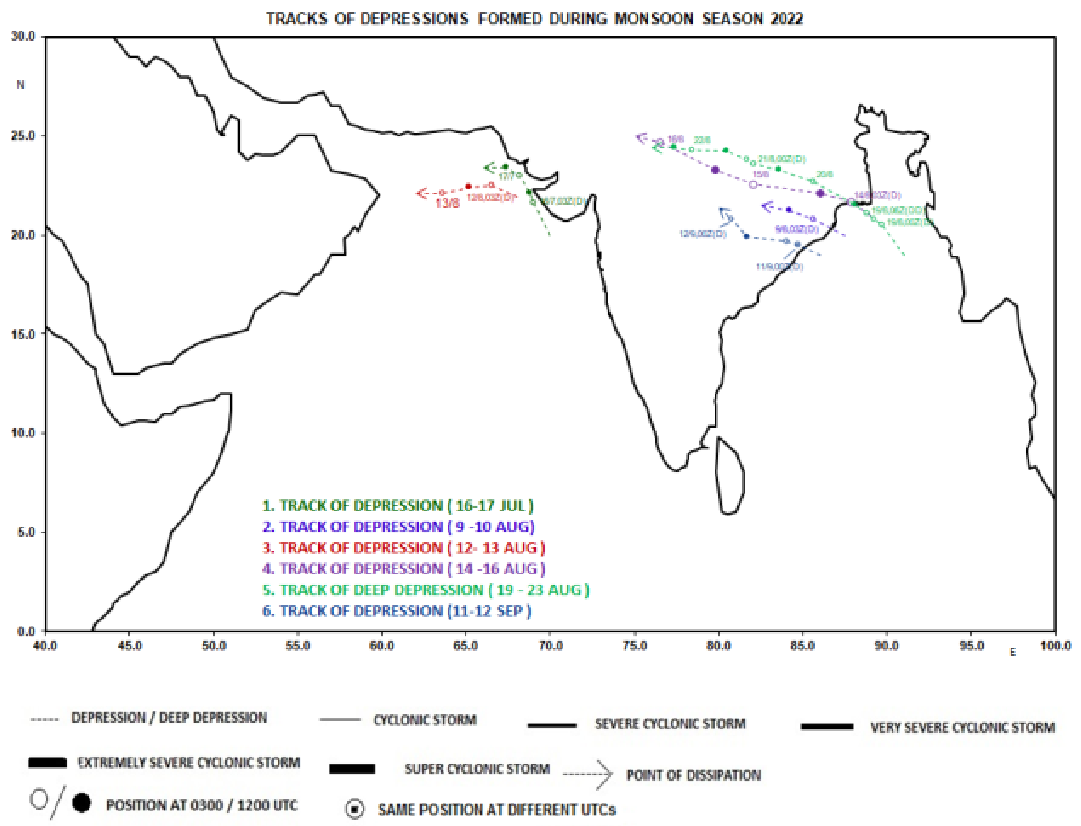
\includegraphics[width=1.1\linewidth, height=0.74\textheight]{images/IMD-report-2022.png}
%                     % 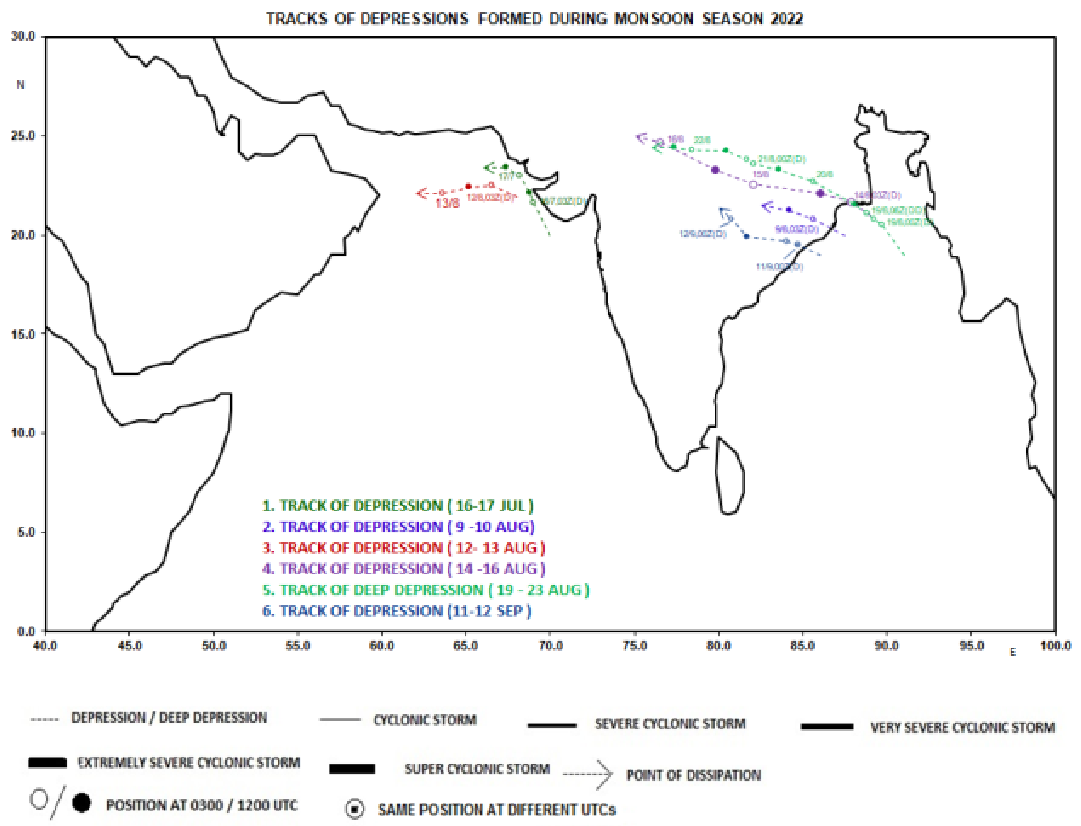
\includegraphics[width=1.12\linewidth, height=0.5\textheight, keepaspectratio]{images/IMD-report-2022.png}
%                 \end{figure}
%             \footnotesize IMD Annual Monsoon report 2022 \footnotemark[10]
%             \end{center}
%         \end{columns}
%
%         \vspace{-0.7cm}
%         \footnotetext[10]{\tiny Source : IMD Annual Monsoon Report 2022 (page 29) \href{https://mausam.imd.gov.in/imd\_latest/contents/ar2022.pdf}{\url{https://mausam.imd.gov.in/imd\_latest/contents/ar2022.pdf}}}
%     \end{center}
% \end{frame}

\subsubsection{Primitive MD detection for 2023}
\begin{frame}[label=tracks2023]{MD Tracks (June-September 2023)}
	\vspace{-0.5cm}
	\begin{center}
		\begin{columns}[T, onlytextwidth]
			\column{0.48\textwidth}
			\begin{center}
				\begin{figure}
					\includegraphics[width=1.1\linewidth]{../version15-with-no-ocean-masking/output_2023/MD_track_2023.png}
				\end{figure}
				\footnotesize Detected MD tracks using ERA5 single level Dataset (2023)
			\end{center}

			\vspace{-0.9cm}
			\column{0.48\textwidth}
			\begin{center}
				\begin{figure}
					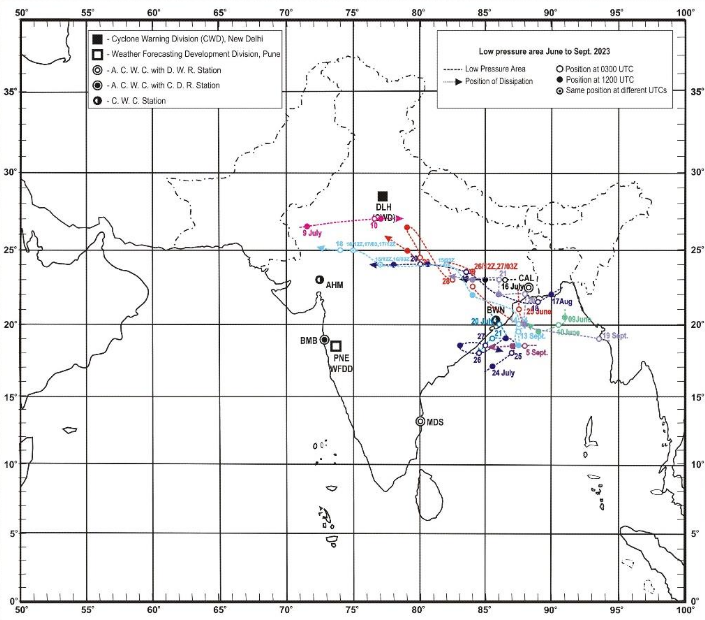
\includegraphics[width=1.1\linewidth, height=0.74\textheight]{images/IMD-report-2023.png}
					% 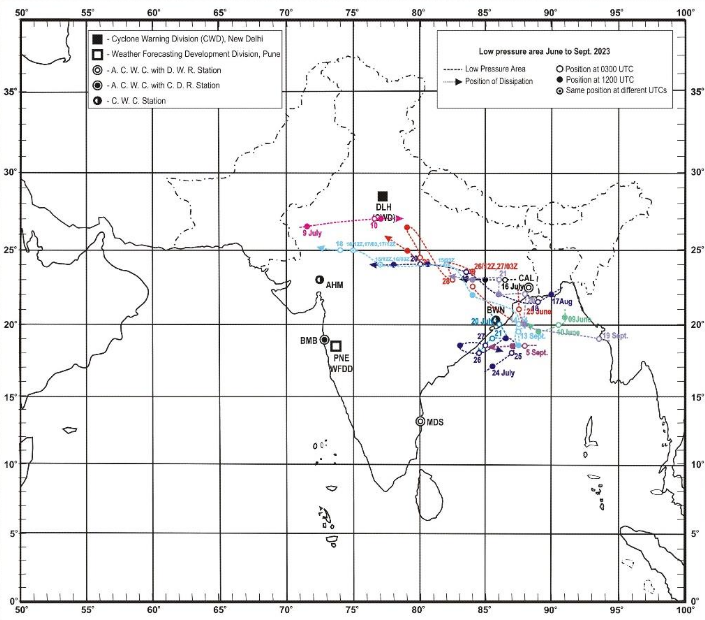
\includegraphics[width=1.12\linewidth, height=0.5\textheight, keepaspectratio]{images/IMD-report-2023.png}
				\end{figure}
				\footnotesize IMD Annual Monsoon report 2023 \footnotemark[10]
			\end{center}
		\end{columns}

		\vspace{-0.6cm}
		\footnotetext[10]{\tiny Source : IMD Annual Monsoon Report 2023 (page 23) \href{https://internal.imd.gov.in/press\_release/20231001\_pr\_2555.pdf}{\url{https://internal.imd.gov.in/press\_release/20231001\_pr\_2555.pdf}}}
	\end{center}
\end{frame}

\subsubsection{Primitive MD detection for 2025}
\begin{frame}[label=tracks2025]{MD Tracks (June-September 2025)}
	\vspace{-0.5cm}
	\begin{center}
		\begin{columns}[T, onlytextwidth]
			\column{0.48\textwidth}
			\begin{center}
				\begin{figure}
					\includegraphics[width=1.1\linewidth]{../version15-with-no-ocean-masking/output_2025/MD_track_2025.png}
				\end{figure}
				\footnotesize Detected MD tracks using ERA5 single level Dataset (2025)
			\end{center}

			\vspace{-0.9cm}
			\column{0.48\textwidth}
			\begin{center}
				\begin{figure}
					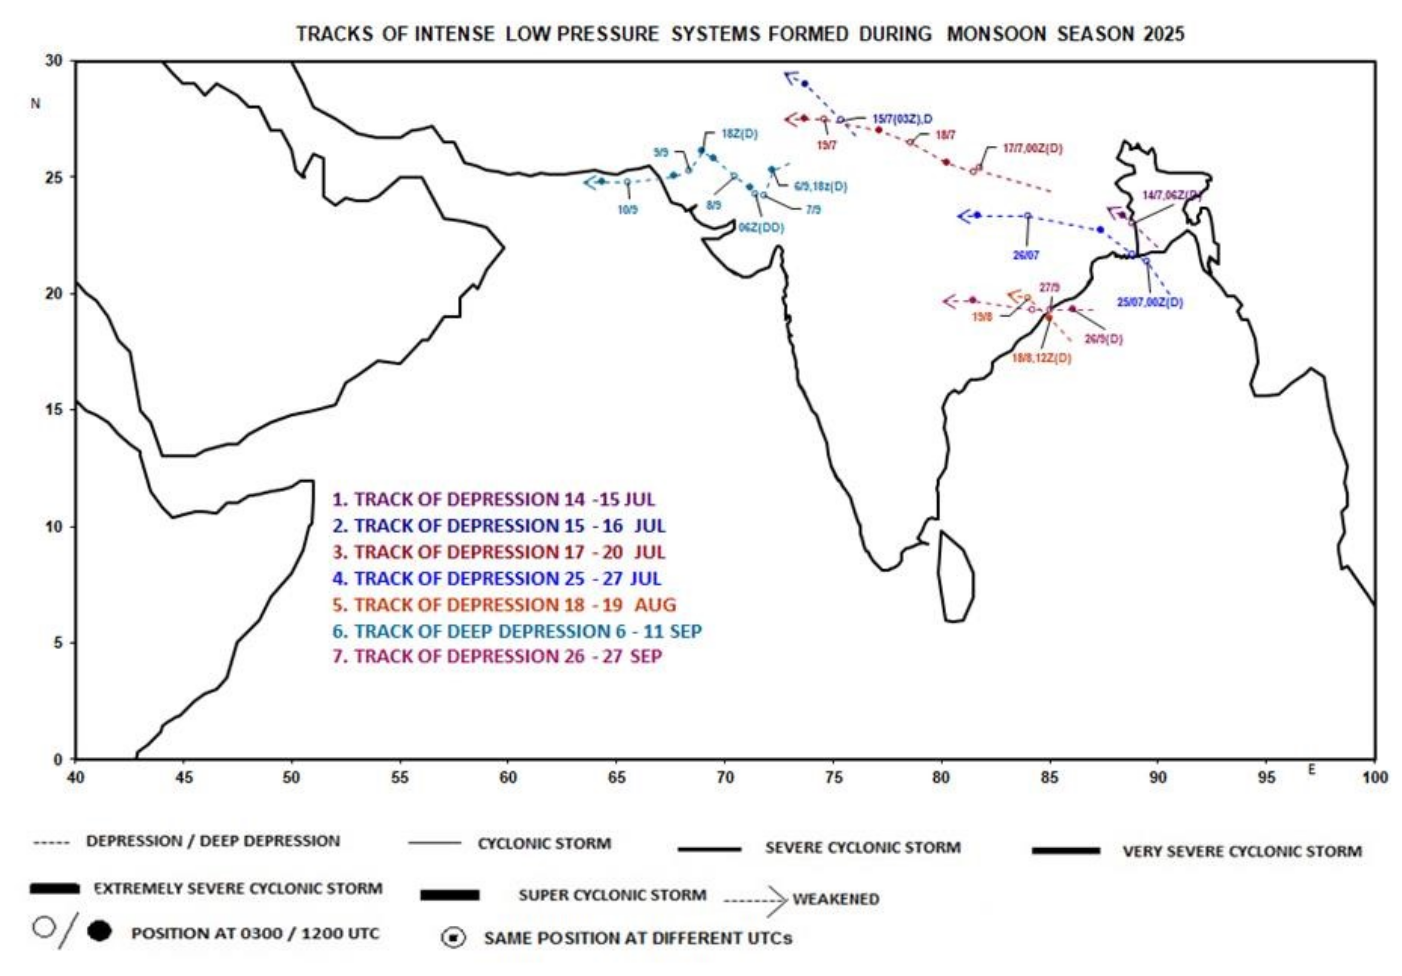
\includegraphics[width=1.1\linewidth, height=0.74\textheight]{images/IMD-report-2025.png}
					% 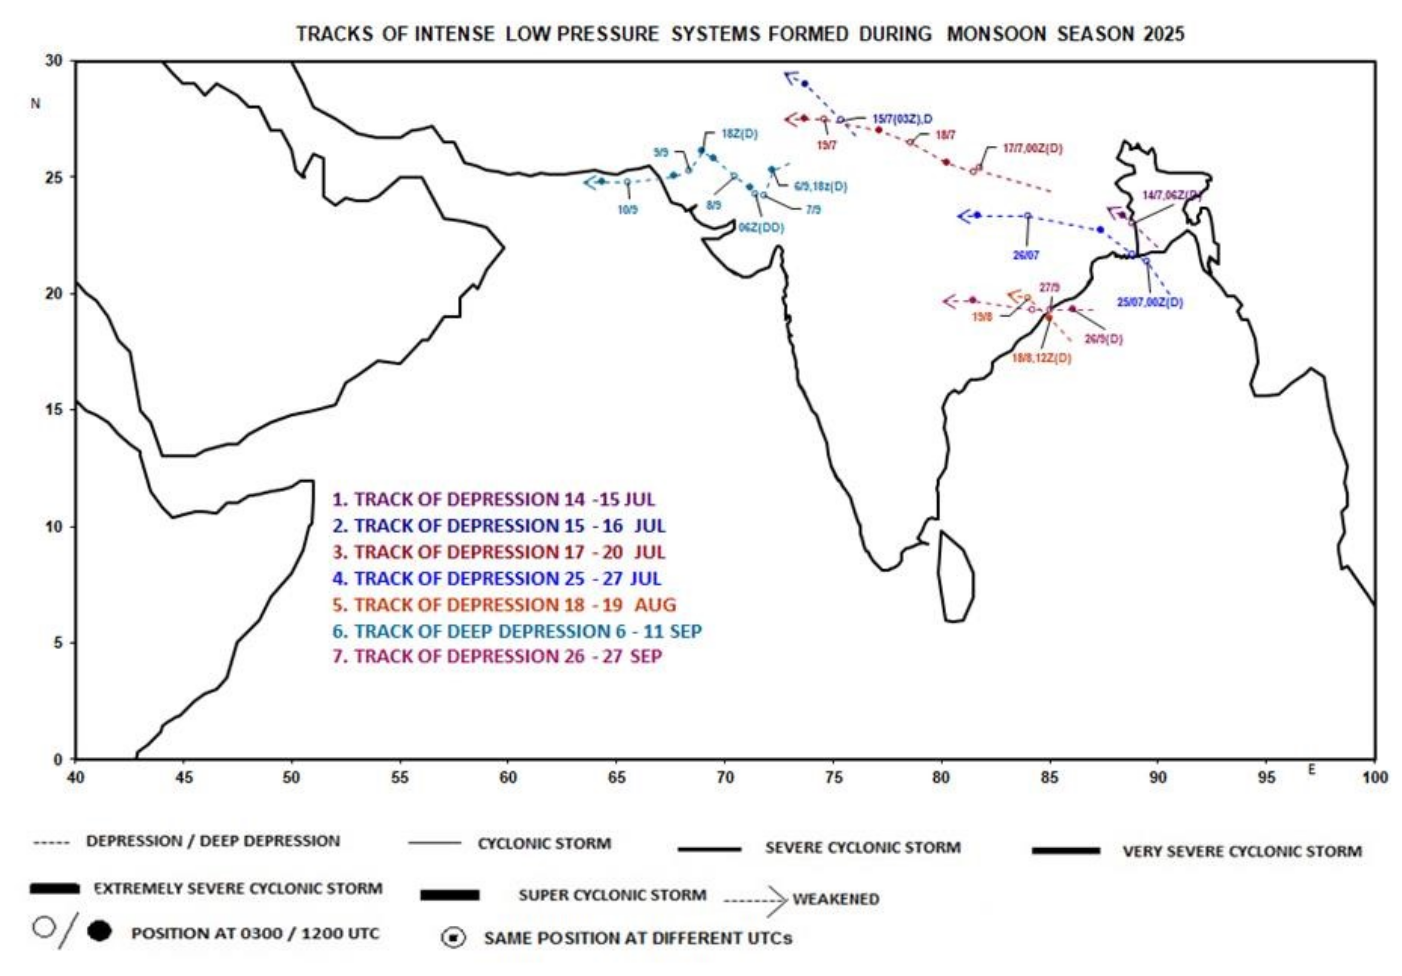
\includegraphics[width=1.12\linewidth, height=0.5\textheight, keepaspectratio]{images/IMD-report-2025.png}
				\end{figure}
				\footnotesize IMD Annual Monsoon report 2025 \footnotemark[10]
			\end{center}
		\end{columns}

		\vspace{-0.6cm}
		\footnotetext[10]{\tiny Source : IMD Annual Monsoon Report 2025 (page 7) \href{https://mausam.imd.gov.in/newdelhi/archive/2025-12-13/press\_release\_en.pdf}{\url{https://mausam.imd.gov.in/newdelhi/archive/2025-12-13/press\_release\_en.pdf}}}
	\end{center}
\end{frame}

\begin{frame}{Final Summary}
	\begin{center}
		\textbf{Why Some Monsoon Depressions Die Over Land While Others Survive?}

		\vspace{0.5cm}
		\textbf{Soil Moisture Determines Monsoon Depression Fate Over Land}

		\vspace{0.5cm}
		\footnotesize
		\begin{tabular}{lll}
			\toprule
			\textbf{Factor}                                                        & \textbf{Role}                       & \textbf{Timescale} \\
			\midrule
			Soil type sets the capacity, BUT elevation sets the infiltration rates & Days to weeks                                            \\
			Pre-landfall SM                                                        & Provides fuel (initial condition)   & Hours              \\
			Coupling strength                                                      & Sustains feedback (dynamic)         & Hours              \\
			Diurnal heating                                                        & Amplifies instability (daily cycle) & Hours              \\
			Memory                                                                 & Maintains persistence (multi-day)   & Days               \\
			\bottomrule
		\end{tabular}

		\vspace{0.3cm}
		\footnotesize
		\textit{All five factors work together. Missing any one limits longevity.}
	\end{center}

	\vspace{0.3cm}
	\textbf{Answer: Soil type and Pre-landfall condition matters as much as the atmosphere (Heat fluxes)}

	\vspace{0.3cm}
	\footnotesize
	\begin{itemize}
		\item Soil type sets the \textbf{capacity}.
		\item Elevation sets the \textbf{infiltration rates} (inversely proportional).
		\item Soil moisture sets the \textbf{fuel} for MD after Landfall weakening.
		\item Precipitation-soil feedback sets the \textbf{efficiency} also for longevity.
	\end{itemize}
\end{frame}
